\documentclass{standalone}
\usepackage{tikz}
\usetikzlibrary{patterns, positioning}
\usepackage[sfdefault]{ClearSans} %% option 'sfdefault' activates Clear Sans as the default text font
\usepackage[T1]{fontenc}

\begin{document}
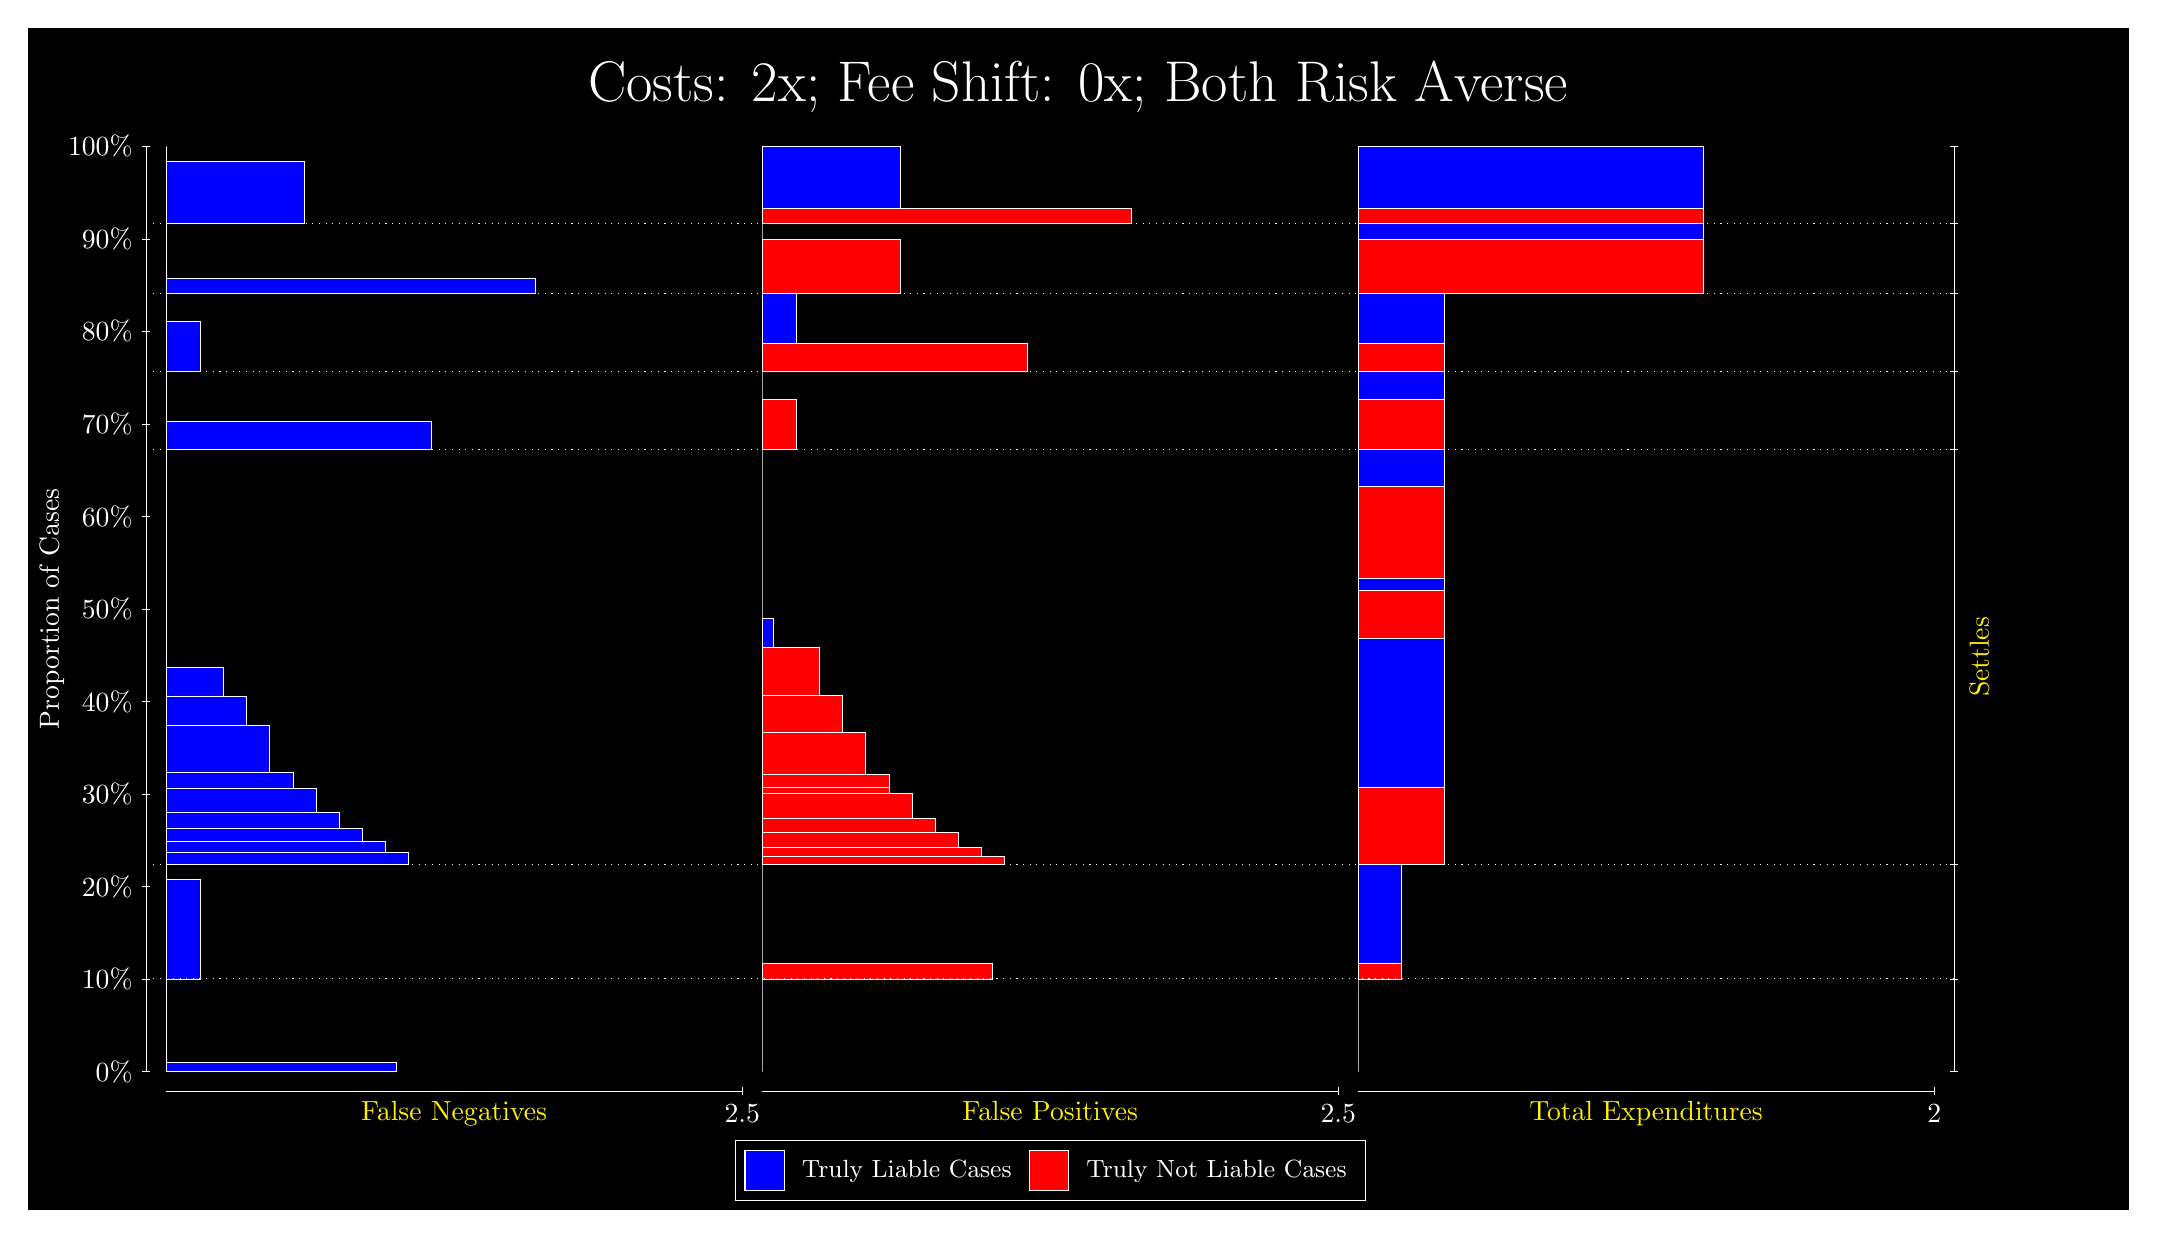
\begin{tikzpicture}
\draw[fill=black] (0,0) rectangle (26.667,15);
\draw[text=white] (0,13.5) rectangle (26.667,15) node[midway] {\huge Costs: 2x; Fee Shift: 0x; Both Risk Averse};
\draw[white, very thin] (1.5,1.75) -- (1.5,13.5);
\node[rotate=90, text=white, anchor=center] at (0.3, 7.625) {Proportion of Cases};
\draw[white, very thin] (1.45,1.75) -- (1.55,1.75);
\node[text=white, anchor=east] at (1.45, 1.75) {0\%};
\draw[white, very thin] (1.45,2.925) -- (1.55,2.925);
\node[text=white, anchor=east] at (1.45, 2.925) {10\%};
\draw[white, very thin] (1.45,4.1) -- (1.55,4.1);
\node[text=white, anchor=east] at (1.45, 4.1) {20\%};
\draw[white, very thin] (1.45,5.275) -- (1.55,5.275);
\node[text=white, anchor=east] at (1.45, 5.275) {30\%};
\draw[white, very thin] (1.45,6.45) -- (1.55,6.45);
\node[text=white, anchor=east] at (1.45, 6.45) {40\%};
\draw[white, very thin] (1.45,7.625) -- (1.55,7.625);
\node[text=white, anchor=east] at (1.45, 7.625) {50\%};
\draw[white, very thin] (1.45,8.8) -- (1.55,8.8);
\node[text=white, anchor=east] at (1.45, 8.8) {60\%};
\draw[white, very thin] (1.45,9.975) -- (1.55,9.975);
\node[text=white, anchor=east] at (1.45, 9.975) {70\%};
\draw[white, very thin] (1.45,11.15) -- (1.55,11.15);
\node[text=white, anchor=east] at (1.45, 11.15) {80\%};
\draw[white, very thin] (1.45,12.325) -- (1.55,12.325);
\node[text=white, anchor=east] at (1.45, 12.325) {90\%};
\draw[white, very thin] (1.45,13.5) -- (1.55,13.5);
\node[text=white, anchor=east] at (1.45, 13.5) {100\%};

\draw[white, very thin] (24.457,1.75) -- (24.457,13.5);
\draw[white, very thin] (24.407,1.75) -- (24.507,1.75);
\node[anchor=west] at (24.407, 1.75) {};
\draw[white, very thin] (24.407,2.9259) -- (24.507,2.9259);
\node[anchor=west] at (24.407, 2.9259) {};
\draw[white, very thin] (24.407,4.3844) -- (24.507,4.3844);
\node[anchor=west] at (24.407, 4.3844) {};
\draw[white, very thin] (24.407,9.6467) -- (24.507,9.6467);
\node[anchor=west] at (24.407, 9.6467) {};
\draw[white, very thin] (24.407,10.644) -- (24.507,10.644);
\node[anchor=west] at (24.407, 10.644) {};
\draw[white, very thin] (24.407,11.634) -- (24.507,11.634);
\node[anchor=west] at (24.407, 11.634) {};
\draw[white, very thin] (24.407,12.517) -- (24.507,12.517);
\node[anchor=west] at (24.407, 12.517) {};
\draw[white, very thin] (24.407,13.5) -- (24.507,13.5);
\node[anchor=west] at (24.407, 13.5) {};

\draw[white, very thin, fill=blue] (1.75,1.75) rectangle (4.6775,1.8737);
\draw[white, very thin, fill=red] (1.75,1.8737) rectangle (1.75,2.9259);
\draw[white, very thin, fill=blue] (1.75,2.9259) rectangle (2.1891,4.1917);
\draw[white, very thin, fill=red] (1.75,4.1917) rectangle (1.75,4.3844);
\draw[white, very thin, fill=blue] (1.75,4.3844) rectangle (4.8239,4.5394);
\draw[white, very thin, fill=blue] (1.75,4.5394) rectangle (4.5312,4.6683);
\draw[white, very thin, fill=blue] (1.75,4.6683) rectangle (4.2384,4.8335);
\draw[white, very thin, fill=blue] (1.75,4.8335) rectangle (3.9457,5.0472);
\draw[white, very thin, fill=blue] (1.75,5.0472) rectangle (3.6529,5.3462);
\draw[white, very thin, fill=blue] (1.75,5.3462) rectangle (3.3602,5.5465);
\draw[white, very thin, fill=blue] (1.75,5.5465) rectangle (3.0674,6.1461);
\draw[white, very thin, fill=blue] (1.75,6.1461) rectangle (2.7746,6.5204);
\draw[white, very thin, fill=blue] (1.75,6.5204) rectangle (2.4819,6.8896);
\draw[white, very thin, fill=red] (1.75,6.8896) rectangle (1.75,9.6467);
\draw[white, very thin, fill=blue] (1.75,9.6467) rectangle (5.1167,10.004);
\draw[white, very thin, fill=red] (1.75,10.004) rectangle (1.75,10.644);
\draw[white, very thin, fill=blue] (1.75,10.644) rectangle (2.1891,11.284);
\draw[white, very thin, fill=red] (1.75,11.284) rectangle (1.75,11.634);
\draw[white, very thin, fill=blue] (1.75,11.634) rectangle (6.4341,11.827);
\draw[white, very thin, fill=red] (1.75,11.827) rectangle (1.75,12.517);
\draw[white, very thin, fill=blue] (1.75,12.517) rectangle (3.5065,13.306);
\draw[white, very thin, fill=red] (1.75,13.306) rectangle (1.75,13.5);
\draw[white, very thin, fill=red] (9.3189,1.75) rectangle (9.3189,2.8021);
\draw[white, very thin, fill=blue] (9.3189,2.8021) rectangle (9.3189,2.9259);
\draw[white, very thin, fill=red] (9.3189,2.9259) rectangle (12.246,3.1185);
\draw[white, very thin, fill=blue] (9.3189,3.1185) rectangle (9.3189,4.3844);
\draw[white, very thin, fill=red] (9.3189,4.3844) rectangle (12.393,4.4774);
\draw[white, very thin, fill=red] (9.3189,4.4774) rectangle (12.1,4.6014);
\draw[white, very thin, fill=red] (9.3189,4.6014) rectangle (11.807,4.7911);
\draw[white, very thin, fill=red] (9.3189,4.7911) rectangle (11.515,4.9667);
\draw[white, very thin, fill=red] (9.3189,4.9667) rectangle (11.222,5.2833);
\draw[white, very thin, fill=red] (9.3189,5.2833) rectangle (10.929,5.3613);
\draw[white, very thin, fill=red] (9.3189,5.3613) rectangle (10.929,5.5296);
\draw[white, very thin, fill=red] (9.3189,5.5296) rectangle (10.636,6.0544);
\draw[white, very thin, fill=red] (9.3189,6.0544) rectangle (10.344,6.5302);
\draw[white, very thin, fill=red] (9.3189,6.5302) rectangle (10.051,7.1415);
\draw[white, very thin, fill=blue] (9.3189,7.1415) rectangle (9.4652,7.5107);
\draw[white, very thin, fill=blue] (9.3189,7.5107) rectangle (9.3189,9.6467);
\draw[white, very thin, fill=red] (9.3189,9.6467) rectangle (9.758,10.286);
\draw[white, very thin, fill=blue] (9.3189,10.286) rectangle (9.3189,10.644);
\draw[white, very thin, fill=red] (9.3189,10.644) rectangle (12.686,10.994);
\draw[white, very thin, fill=blue] (9.3189,10.994) rectangle (9.758,11.634);
\draw[white, very thin, fill=red] (9.3189,11.634) rectangle (11.075,12.324);
\draw[white, very thin, fill=blue] (9.3189,12.324) rectangle (9.3189,12.517);
\draw[white, very thin, fill=red] (9.3189,12.517) rectangle (14.003,12.71);
\draw[white, very thin, fill=blue] (9.3189,12.71) rectangle (11.075,13.5);
\draw[white, very thin, fill=red] (16.888,1.75) rectangle (16.888,2.8021);
\draw[white, very thin, fill=blue] (16.888,2.8021) rectangle (16.888,2.9259);
\draw[white, very thin, fill=red] (16.888,2.9259) rectangle (17.437,3.1185);
\draw[white, very thin, fill=blue] (16.888,3.1185) rectangle (17.437,4.3844);
\draw[white, very thin, fill=red] (16.888,4.3844) rectangle (17.986,5.3613);
\draw[white, very thin, fill=blue] (16.888,5.3613) rectangle (17.986,7.2508);
\draw[white, very thin, fill=red] (16.888,7.2508) rectangle (17.986,7.8621);
\draw[white, very thin, fill=blue] (16.888,7.8621) rectangle (17.986,8.0172);
\draw[white, very thin, fill=red] (16.888,8.0172) rectangle (17.986,9.186);
\draw[white, very thin, fill=blue] (16.888,9.186) rectangle (17.986,9.6467);
\draw[white, very thin, fill=red] (16.888,9.6467) rectangle (17.986,10.286);
\draw[white, very thin, fill=blue] (16.888,10.286) rectangle (17.986,10.644);
\draw[white, very thin, fill=red] (16.888,10.644) rectangle (17.986,10.994);
\draw[white, very thin, fill=blue] (16.888,10.994) rectangle (17.986,11.634);
\draw[white, very thin, fill=red] (16.888,11.634) rectangle (21.279,12.324);
\draw[white, very thin, fill=blue] (16.888,12.324) rectangle (21.279,12.517);
\draw[white, very thin, fill=red] (16.888,12.517) rectangle (21.279,12.71);
\draw[white, very thin, fill=blue] (16.888,12.71) rectangle (21.279,13.5);
\draw[white, dotted] (1.5,2.9259) -- (24.457,2.9259);
\draw[white, dotted] (1.5,4.3844) -- (24.457,4.3844);
\draw[white, dotted] (1.5,9.6467) -- (24.457,9.6467);
\draw[white, dotted] (1.5,10.644) -- (24.457,10.644);
\draw[white, dotted] (1.5,11.634) -- (24.457,11.634);
\draw[white, dotted] (1.5,12.517) -- (24.457,12.517);
\draw[white, very thin] (1.75,1.5) -- (9.0689,1.5);
\node[text=yellow, anchor=north] at (5.4094, 1.5) {False Negatives};
\draw[white, very thin] (9.0689,1.45) -- (9.0689,1.55);
\node[text=white, anchor=north] at (9.0689, 1.45) {2.5};

\draw[white, very thin] (9.3189,1.5) -- (16.638,1.5);
\node[text=yellow, anchor=north] at (12.978, 1.5) {False Positives};
\draw[white, very thin] (16.638,1.45) -- (16.638,1.55);
\node[text=white, anchor=north] at (16.638, 1.45) {2.5};

\draw[white, very thin] (16.888,1.5) -- (24.207,1.5);
\node[text=yellow, anchor=north] at (20.547, 1.5) {Total Expenditures};
\draw[white, very thin] (24.207,1.45) -- (24.207,1.55);
\node[text=white, anchor=north] at (24.207, 1.45) {2};



\node[text=yellow, centered, rotate=90] at (24.777, 7.0156) {Settles};





\draw (12.978300999999998,1.5) node[draw=none] (baseCoordinate) {};
\begin{scope}[align=center]
        \matrix[scale=0.5, draw=white, below=0.5cm of baseCoordinate, nodes={draw}, column sep=0.1cm]{
            \node[rectangle, draw, minimum width=0.5cm, minimum height=0.5cm, fill=blue] {}; &
            \node[draw=none, font=\small, text=white] (B) {Truly Liable Cases}; &
            \node[rectangle, draw, minimum width=0.5cm, minimum height=0.5cm, fill=red] {}; &
            \node[draw=none, font=\small, text=white] (B) {Truly Not Liable Cases}; \\
            };
\end{scope}

\end{tikzpicture}
\end{document}